\documentclass[tikz,border=5pt]{standalone}
\usepackage{amsmath}
\usetikzlibrary{arrows.meta,positioning}
\begin{document}
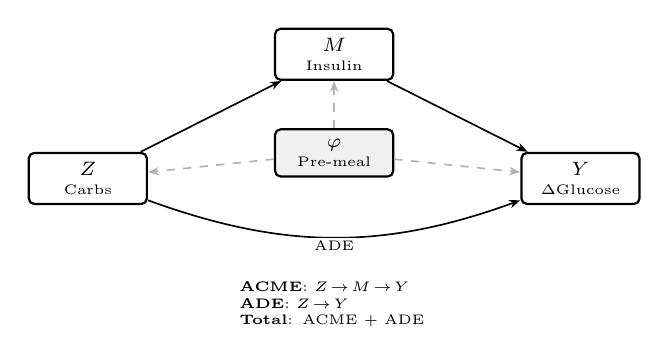
\begin{tikzpicture}[
    node distance=1cm and 1.4cm,
    block/.style={
        rectangle, rounded corners=2pt, draw=black, thick,
        minimum width=1.5cm, minimum height=0.6cm,
        font=\scriptsize, align=center, fill=white
    },
    arr/.style={-{Stealth[length=4pt]}, semithick},
    lbl/.style={font=\tiny, fill=white, inner sep=1pt}
]
% Nodes -- triangle with phi below
\node[block] (Z) {$Z$\\[-1pt]{\tiny Carbs}};
\node[block, above right=0.9cm and 1.6cm of Z] (M) {$M$\\[-1pt]{\tiny Insulin}};
\node[block, below right=0.9cm and 1.6cm of M] (Y) {$Y$\\[-1pt]{\tiny $\Delta$Glucose}};
\node[block, below=0.6cm of M, fill=gray!12] (phi) {$\varphi$\\[-1pt]{\tiny Pre-meal}};
% Causal edges
\draw[arr] (Z) -- (M);
\draw[arr] (M) -- (Y);
\draw[arr] (Z) to[bend right=20] node[lbl, below] {ADE} (Y);
% Confounder arrows (dashed)
\draw[arr, dashed, gray!60] (phi) -- (Z);
\draw[arr, dashed, gray!60] (phi) -- (M);
\draw[arr, dashed, gray!60] (phi) -- (Y);
% Legend
\node[font=\tiny, anchor=north, text width=2.4cm, align=left]
  at ([yshift=-1.2cm]phi.south) {%
    \textbf{ACME}: $Z \!\to\! M \!\to\! Y$\\
    \textbf{ADE}: $Z \!\to\! Y$\\
    \textbf{Total}: ACME $+$ ADE};
\end{tikzpicture}
\end{document}
